% Scenario: Upgrading Cloud Infrastructure for High Demand
\begin{table}[H]
    \centering
    \begin{tabularx}{\textwidth}{@{} lX @{}}
    \toprule
    \textbf{Aspect} & \textbf{Details} \\
    \midrule
    Source & TrIP system experiencing a surge in demand due to a new university opening at a station. \\
    Stimulus & Passenger numbers have more than quadrupled, causing performance delays during rush hours. \\
    Artifact & The deployment of the TrIP system across public cloud servers and private cloud servers. \\
    Response & The system's cloud infrastructure is updated to leverage elastic scaling capabilities. Load balancers distribute the increased traffic efficiently, and additional computing resources are allocated to handle the high load, particularly for route optimization and payment processing components. \\
    Measure & Post-update, the TrIP system handles a fourfold increase in user load with response times reduced by 70\%, ensuring that all passengers complete their transactions and receive route information within 2 seconds, even during peak rush hours. \\
    \bottomrule
    \end{tabularx}
    \caption{Scenario for Performance - Cloud Infrastructure Scaling}
    \label{table:performance_scaling}
\end{table}

% Scenario: Reinforcement of Data Security and Privacy Protocols
\begin{table}[H]
    \centering
    \begin{tabularx}{\textwidth}{@{} lX @{}}
    \toprule
    \textbf{Aspect} & \textbf{Details} \\
    \midrule
    Source & TrIP system architecture analysis in response to a competitor's security breach. \\
    Stimulus & The need to verify and bolster the security measures in place to protect passenger data. \\
    Artifact & Deployment architecture of the TrIP system with a focus on data servers and encryption protocols. \\
    Response & The system utilizes advanced encryption for data at rest and in transit within private cloud servers. Access controls are strictly enforced, ensuring only authenticated and authorized components interact with sensitive data. Periodic security audits and real-time intrusion detection systems are in place to monitor and immediately respond to any unauthorized access attempts. \\
    Measure & Security tests confirm no data leakage, and the system's compliance with the latest privacy regulations is validated by a third-party security firm, ensuring that the board and tycoons have verifiable assurance of the system's security measures. \\
    \bottomrule
    \end{tabularx}
    \caption{Scenario for Security - Privacy and Data Protection}
    \label{table:security_privacy}
\end{table}


\section{Deployment Viewpoint}
We start discussing the deployment viewpoint by analyzing stakeholder concerns that need to be addressed.
We individuated the following user stories:
\begin{itemize}
    \item User stories TODO
\end{itemize}

As a consequence, we decided to prioritize Quality Attributes for this view as indicated in Table~\ref{tab:deployment_view}.
\begin{table}[h!]
    \centering
    \resizebox{\textwidth}{!}{%
    \begin{tabular}{|l|c|c|c|c|c|c|c|c|c|}
      \hline
      & Usability & Performance & Security & Modifiability & Cost Efficiency & Availability & Safety & Integrability & Maintainability \\
      \hline
      Deployment View & 
       & % Usability
      \cellcolor{gray!90}X & % Performance (1st priority)
      \cellcolor{gray!60}X & % Security (3rd priority)
       & % Modifiability
       & % Cost Efficiency
       & % Availability (2nd priority)
       & % Safety
       & % Integrability
       \\ % Maintainability
      \hline
    \end{tabular}
    }
    \caption{Deployment View Prioritized Quality Attributes}
    \label{tab:deployment_view}
\end{table}

\subsection{View: Scanning procedure}
\subsubsection{Model}
\begin{figure}[H]
    \centering
    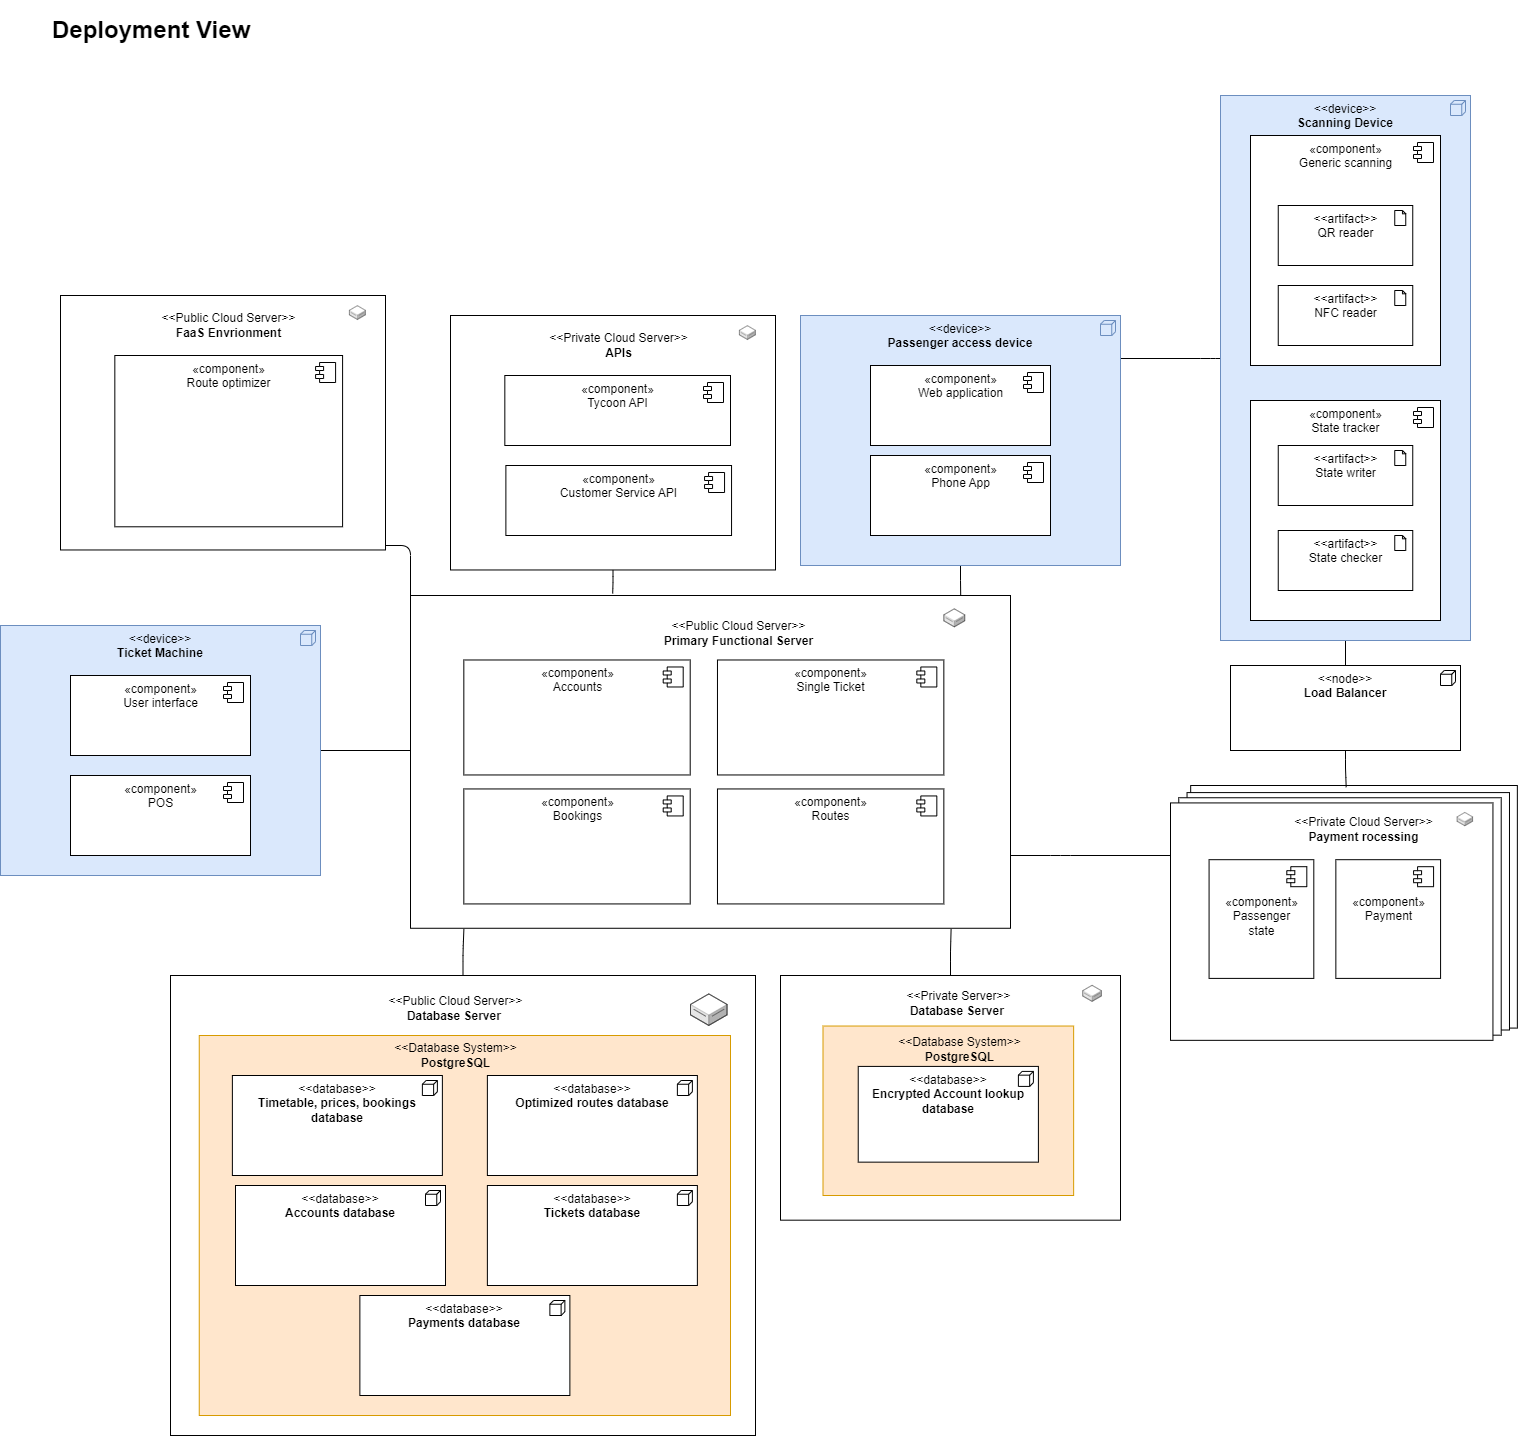
\includegraphics[width=\textwidth]{drawings/views_final_version/deployment_view.png}
    \caption{Deployment view related to the scanning procedure.}
    \label{fig:deployment_view_scanning}
\end{figure}

\subsubsection{Description}
The deployment view diagram illustrates the TrIP system's architecture, showing components distributed across public and private cloud servers. Public cloud servers house the FaaS Environment for route optimization, a Terminal with Customer Service API, and the Primary Functional Server hosting Accounts, Single Ticket, Bookings, and Routes components. Devices for passenger access, such as web and phone apps, interface with scanning devices like QR and NFC readers, managed by state trackers and checkers.

The ticket machine interfaces include User Interface and POS components. Database servers in the public cloud manage the PostgreSQL databases for Timetables, Prices, Bookings, Optimized Routes, Accounts, Tickets, and Payments. The private cloud server secures the Encrypted Account Lookup database. A Load Balancer ensures efficient traffic management.

Payment processing, crucial for managing Passenger State and payments, is securely handled in the private cloud, emphasizing the system's focus on security and reliable transaction handling. 
\subsubsection{Glossary of Elements}

\begin{table}[H]
    \centering
    \caption{Glossary for the Deployment View of the TrIP SYSTEM.}
    \label{tab:deployment_view_glossary}
    \begin{tabularx}{\textwidth}{@{}lXX@{}} % Corrected to have three columns
    \toprule
    \textbf{Component} & \textbf{Description} & \textbf{Hosted On} \\
    \midrule
    FaaS Environment & Provides a platform for executing backend functions in a serverless architecture, such as route optimization. & Public Cloud Servers \\
    Tycoon API & Interfaces allowing tycoons' software and systems to communicate with the TrIP system. & Private Cloud Servers \\
    Customer Service API & Facilitates customer service operations by providing data access and manipulation capabilities. & Private Cloud Servers \\
    Passenger Access Device & Equipment that passengers interact with to access the system, like ticket validation and purchases. & Terminal, App, Website \\
    Ticket Machine & Physical machines where passengers can purchase tickets and manage their bookings. & Station Locations \\
    Scanning Device & Tools used for reading ticket information, necessary for entry validation and passenger tracking. & Entry/Exit Gates \\
    QR Reader & Specialized scanners that interpret QR codes on tickets for entry validation or information retrieval. & Scanning Devices \\
    NFC Reader & Contactless devices that read NFC tags for authentication and ticket validation. & Passenger Access Devices \\
    Timetable, Prices, Bookings Database & Stores all relevant data for scheduling, pricing, and passenger bookings. & Public Cloud Servers \\
    Optimized Routes Database & Contains data on the most efficient routes calculated by the optimization algorithms. & Public Cloud Servers \\
    Accounts Database & Manages passenger account information, including subscription details and personal data. & Public Cloud Servers \\
    Tickets Database & Holds data related to ticket sales, validations, and historical transactions. & Public Cloud Servers \\
    Payments Database & Processes and records all payment transactions within the system. & Public Cloud Servers \\
    Encrypted Account Lookup Database & A secure database that stores sensitive account information, accessible only through authorized queries. & Private Cloud Servers \\
    \bottomrule
    \end{tabularx}
\end{table}
\subsubsection{Analysis on Perspectives}

\paragraph{Scenarios}
\scenarioOneDeployment
\scenarioTwoDeployment

In the Deployment Viewpoint, the TRiP system's architecture is strategically distributed across a combination of cloud-based and localized servers to optimize for both \textit{performance} and \textit{security}, critical attributes for the robustness and reliability of the system.

The TRiP system's deployment on cloud servers is engineered to enhance \textit{performance}. The public cloud servers provide a scalable Fast Environment for handling dynamic user demands and instantaneous Route Optimization, ensuring that the most efficient paths are always available to the user. This optimization is further supported by Load Balancers, which are essential in managing network traffic by distributing workloads evenly, thereby preventing any server from becoming a bottleneck and ensuring a smooth user experience. 

For \textit{security}, the system employs private cloud servers, where sensitive components such as the Encrypted Account Lookup Database are hosted. The encryption of this database is a crucial security measure, safeguarding personal and travel data against unauthorized access. 